\section{Common part}
\subsection{Anti-aliasing}
In computer graphics using raster images can lead to "stairstepping" or aliasing. Aliasing can generally be replaced by noise, if the ray origins are randomly placed inside a pixel. Fully random placement of the ray-starting point is not optimal, as the randomly distributed pixels can clump together and leave some areas poorly sampled. Therefore each pixel is subdivided into sub-areas and each sub-area is given one sample. This is called jittered sampling. 

\subsection{Area Lights}
In contrast to point lights, area lights have a surface. In order to solve the rendering equation for scenes lit by area lights, the area form is considered \footnote{Ray Tracing from the ground up page 329}:
\begin{equation}
\mathbf{L}_r(\mathbf{p},\mathbf{\omega}_0) = \int_{A_{\text{light}}} f_r(\mathbf{p},\mathbf{\omega}_i,\mathbf{\omega}_0) \mathbf{L}_e(\mathbf{p}',-\mathbf{\omega}_i)V(\mathbf{p},\mathbf{p}')G(\mathbf{p},\mathbf{p}')dA_{\mathbf{p}'}
\end{equation}
The above equation allows it to find the outgoing light at a primary ray intersection point $\mathbf{p}$. Given the reflection orientation vector $\mathbf{\omega}_0$ and the incoming light direction $\mathbf{\omega}_i = (\mathbf{p} - \mathbf{p}') / \|\mathbf{p} - \mathbf{p}'\|$. The visibility function $V(\mathbf{p}',\mathbf{p})$ is one if point $\mathbf{p}$ is visible from point $\mathbf{p}'$ and zero if not. The geometry term $G$ is given by:
\begin{equation}
G = \frac{cos (\theta_i) cos (\theta')}{\| \mathbf{p}' - \mathbf{p}\| ^ 2}
\end{equation}  
With $cos (\theta_i), cos (\theta')$ given by $\mathbf{n}_\mathbf{p} ^ T \mathbf{\omega}_i$ and $\mathbf{n}^{T}_{\mathbf{p}'} (-\mathbf{\omega}_i)$ respectively. Finally $\mathbf{p}'$ must be a random point within the area light source.
The solution of the rendering equation can be estimated by using Monte-Carlo integration:
\begin{equation}
\mathbf{L}_r(\mathbf{p},\mathbf{\omega}_0) \approx \frac{1}{n_s} \sum_{j=1}^{n_s} \frac{f_r(\mathbf{p},\mathbf{\omega}_{i,j},\mathbf{\omega}_0) \mathbf{L}_e(\mathbf{p}',-\mathbf{\omega}_{i,j})V(\mathbf{p},\mathbf{p}_j')G(\mathbf{p},\mathbf{p_j}')}{p(\mathbf{p}')}
\end{equation}
Here $n_s$ denotes the number of samples, and $p(\mathbf{p}')$ the probability density function. The simplest choice is to distribute the samples uniformly which leads to $p(\mathbf{p}') = \frac{1}{A_l}$. A scene with a spherical and planar light source is shown in figure~\ref{fig:borgEarth}. Using area light sources leads to smooth shadows, like those caused by the cubes on the earth's surface. 


\begin{figure}
\centering
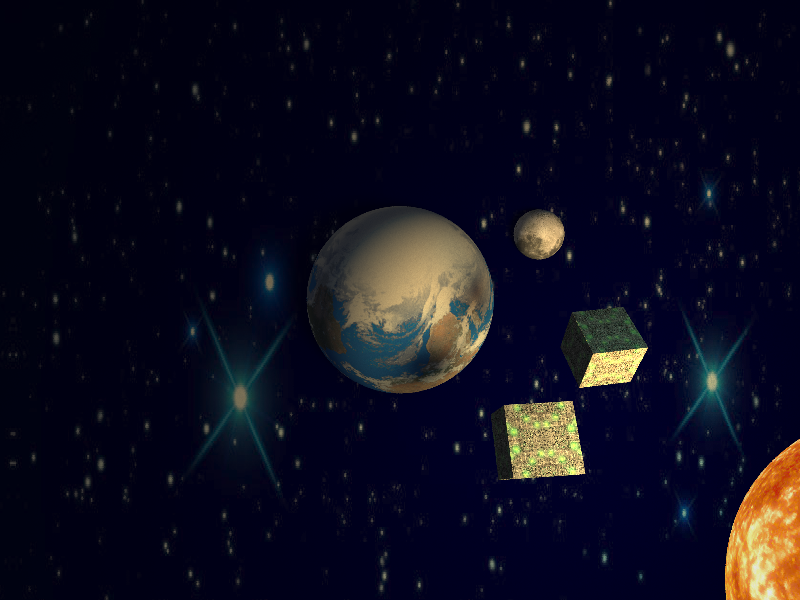
\includegraphics[width=0.45\linewidth]{./img/borgEarth3}
\caption{A spherical area light causing smooth shadows on a sphere}
\label{fig:borgEarth}
\end{figure}
\begin{figure}
\centering
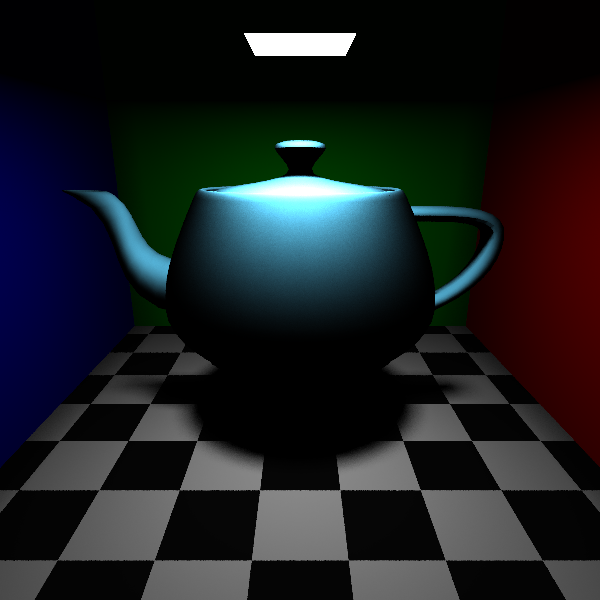
\includegraphics[width=0.45\linewidth]{./img/areaTeapot}
\caption{A rectangular area light illuminating the Utah teapot}
\label{fig:areaTeapot}
\end{figure}


\section{Special effects}
\subsection{Normal Mapping}
In order to add additional normal information or speed up the rendering of wavefront objects, normal data can be loaded from a file. The normal-information is coded as:
\begin{align*}
c_r = 0.5 + 0.5 \cdot n_x \\
c_g = 0.5 + 0.5 \cdot n_y \\
c_b = 0.5 + 0.5 \cdot n_z
\end{align*}
which can be transformed back using:
\begin{align}
n_x = -1.0 + 2*(c_r/255) \\
n_y = -1.0 + 2*(c_g/255) \\
n_z = -1.0 + 2*(c_b/255)
\end{align}
The normal information can then be used for rendering purposes. In case of the Stanford dragon shown in figure~\ref{fig:dragonNormlMap} it took 32s for the high resolution mesh and 6.02s for the low resolution mesh with normal map to produce the same result. 
\begin{figure}
\centering

\includegraphics[width=0.33\linewidth]{./img/dragonHighResMap}

\includegraphics[width=0.33\linewidth]{./img/dragonNormlMap}
\caption{Stanford-Dragon on plane rendered using a high resolution mesh (left) and low resolution mesh with normal map(right).}
\label{fig:dragonNormlMap}
\end{figure}


\subsection{Physical materials}
An important factor in improving the quality of the rendered images is the bidirectional reflectance distribution function (brdf) $f_r(\mathbf{p},\mathbf{\omega}_i,\mathbf{\omega}_0)$. The brdf-model may be split into a diffuse and specular component
\begin{equation}
f_r(\mathbf{p},\mathbf{\omega}_i,\mathbf{\omega}_0) = f_d(\mathbf{p},\mathbf{\omega}_i) + \rho_s f_s(\mathbf{p},\mathbf{\omega}_i,\mathbf{\omega}_0).
\end{equation}
In this project a lambertian
\begin{equation}
f_d(\mathbf{p},\mathbf{\omega}_i) = \frac{\rho_d}{\pi} cos(\theta_i)
\end{equation}
model is used for diffuse part. $\theta_i$ denotes the angle between incoming light and surface normal. The cosine term can be computed using $\mathbf{n}_{\mathbf{p}}^T \mathbf{\omega}_i = cos(\theta_i)$.  
For the specular part a Phong reflection model 
\begin{equation}
f_s(\mathbf{p},\mathbf{\omega}_i,\mathbf{\omega}_0) = \rho_s (\mathbf{r}^T \mathbf{\omega}_0)^e
\end{equation}
is considered.\footnote{Ray Tracing from the ground up page 281} The vector $r$ denotes the mirror reflection direction.  Furthermore a Cook-Torrance model for the specular part has been implemented. This model is taken from their original 1982 publication: \footnote{A Reflectance Model for Computer Graphics, Robert L. Cook, Kenneth E. Torrance, ACM Transactions on Graphics, Vol. 1, No. 1, January 1982, Pages 7-24}
\begin{align}
\mathbf{h} &= \frac{\mathbf{c} + \mathbf{\omega}_i}{\| \mathbf{c} + \mathbf{\omega}_i \|} \\
c & = \mathbf{c}^T \mathbf{h} \\
g &=  \sqrt{n*n + c*c - 1} \\
n &= \frac{1 + \sqrt{f_0}}{1 - \sqrt{f_0}} \\
F &= \frac{1}{2} \frac{(g - c)^2}{(g + c)^2} (1 + \frac{[c (g + c) - 1]^2}{[c (g - c) + 1]^2}) \\
\alpha &= \cos^{-1}(\mathbf{h}^T \mathbf{n}_\mathbf{p}) \\
D &= \frac{1}{m^2 cos^4(\alpha)}e^{[-(\tan(\alpha)/m)]^2} \\
G &= \min(1,
     \frac{2 (\mathbf{n}_\mathbf{p}^T \mathbf{h})(\mathbf{n}_\mathbf{p}^T \mathbf{c})  }{(\mathbf{c}^T \mathbf{h})}),
     \frac{2 (\mathbf{n}_\mathbf{p}^T \mathbf{h})(\mathbf{n}_\mathbf{p}^T \mathbf{\omega}_i)  }{(\mathbf{c}^T \mathbf{h})}) \\
f_s(\mathbf{p},\mathbf{\omega}_i,\mathbf{c}) &= \frac{\rho_s}{\pi}
 \frac{DG}{(\mathbf{n}_{\mathbf{p}}^T \mathbf{\omega}_i)(\mathbf{n}_{\mathbf{p}}^T \mathbf{c})} F(c,g) \\
\end{align} 
The model depends on the two input parameters $f_0$ and $m$ as well as the scaling factor $\rho_s$. The first input is the value of the Fresnel-equation at normal incidence. The second is the root mean square slope $m$ of assumed material facets. The smaller both parameters become the less mirror like will the resulting material will be. The vectors $\mathbf{c,\omega_i}$ point to the camera and the light source respectively.
The vector $\mathbf{h}$ represents the normalized vector in the direction of the angular bisector of the view and light orientation vectors.
The $c$ variable stands for the cosine of the angle between $\mathbf{c}$ and $\mathbf{h}$ or $\omega_i$ and $\mathbf{h}$. 
The Fresnel term $F$ determines how light is reflected from each of the assumed smooth micro-facets. 
A facet slope distribution function $D$ is used. This term depends on the angle between $\mathbf{n_p}$ and $\mathbf{h}$ called $\alpha$.
Finally the geometric attenuation factor $G$ is the last term required to compute the Cook-Torrance BRDF.
\begin{figure}
\centering
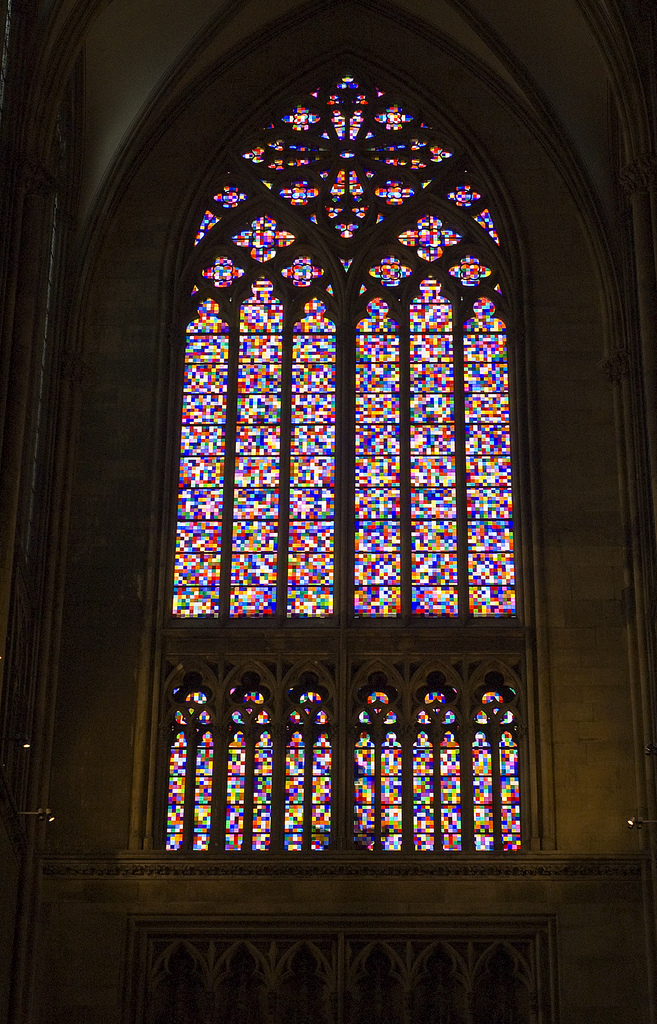
\includegraphics[width=0.25\linewidth]{./img/Richter_window_Cologne_Cathedral}
\includegraphics[width=0.25\linewidth]{./img/Kölner_Dom_Richter_Fenster}
\caption{Gerhard Richter's southern wing main window of the cologne cathedral consisting of 11.500 pixels colored using 72 different colors and pseudo-randomly arranged. On the right the lighting effect of the window on the cathedral floor can be seen.}
\label{fig:Richter_window_Cologne_Cathedral}
\end{figure}
\begin{figure}
\centering
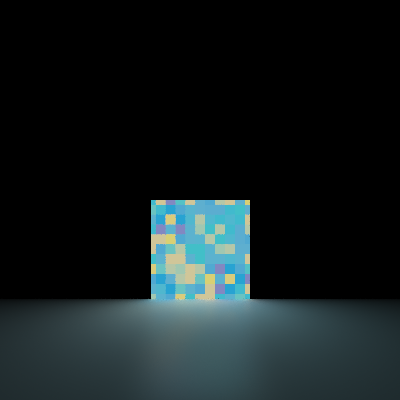
\includegraphics[width=0.3\linewidth]{./img/ph3}
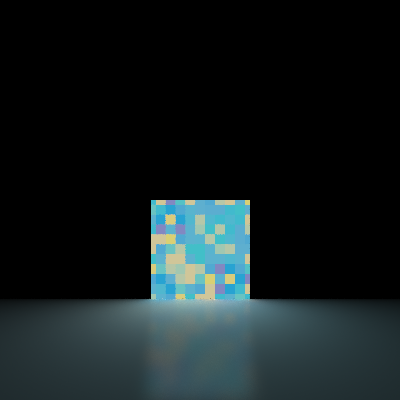
\includegraphics[width=0.3\linewidth]{./img/ph2}
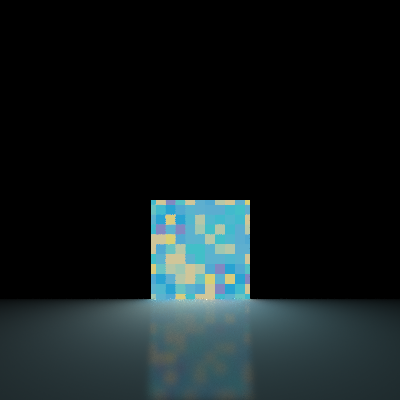
\includegraphics[width=0.3\linewidth]{./img/ph1}
\caption{Importance sampling of Phong's specular reflection model using $e = 100$(left), $e = 500$(middle), $e = 2000$(right). In all cases $\rho_d =0.8$ and $\rho_s = 0.2$}
\label{fig:phongRichter}
\end{figure}
\begin{figure}
\centering
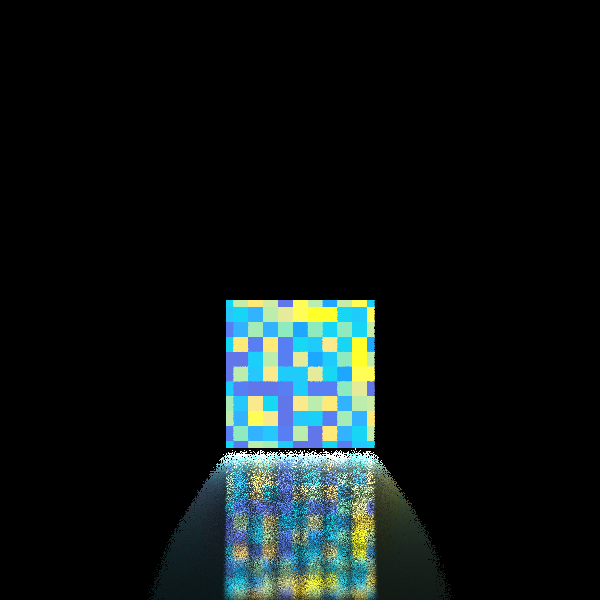
\includegraphics[width=0.3\linewidth]{./img/ct1}
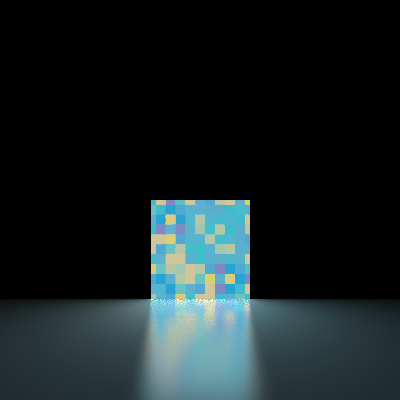
\includegraphics[width=0.3\linewidth]{./img/ct2}
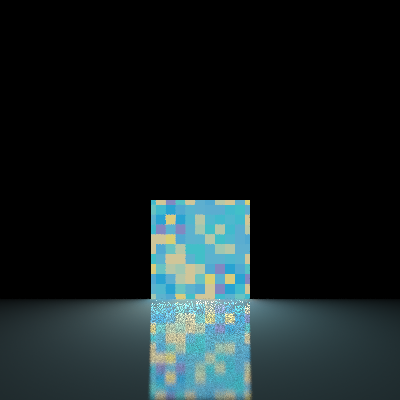
\includegraphics[width=0.3\linewidth]{./img/ct3}
\caption{Scenes computed using Cook-Torrance specular reflection models with parameters $f_0 =0.0366, m = 0.276$ (left),  $f_0 = 0.025, m = 0.076$(middle),  $f_0 = 0.03, m = 0.01$(right). In all cases $\rho_s = 0.2$ and $\rho_d = 0.8$}
\label{fig:CTRichter}
\end{figure}
Gerhard Richter's design of the cologne cathedral's south window and the light effects it produces is shown in figure~\ref{fig:Richter_window_Cologne_Cathedral}. Inspired by the design a rectangular light source with pseudo-randomly distributed squares has been created. This area light source is placed at a ninety degree angle on top of a floor plane. The Specular brdf-component of the floor plane will be varied. First Phong's model is used. 

Results are shown in figure~\ref{fig:phongRichter}. It can be observed that the larger the Phong-exponent $e$ is chosen, the more pronounced the reflection becomes. 
Which makes sense as with larger values for $e$ the set of possible incoming light  vectors at $\mathbf{p}$ with large specular contributions becomes smaller and smaller. Therefore the largest specular contributions come from only a small set of sample points $\mathbf{p'}$ on the light source, which are close to each other. Therefore one expects to see more detailed reflections for larger values of $e$.   \\

In the images shown in figure~\ref*{fig:CTRichter}, the Phong model, has been replaced with a Cook-Torrance model for specular reflection. It can be observed that the larger $m$ is chosen the less visible reflection details become. Which is to be expected as $m$ models the root mean square slope of model material facets, and the larger these slopes are the more bumpy and therefore less mirror like the material will be.

\subsection{Importance Sampling}
In oder to  reduce the amount of samples required to come close to a decent approximation of the solution importance sampling is used. It's key concept is to distribute the sample points $\mathbf{p}'$ on the light source according to their contribution to the solution, important areas of the light should be sampled more often than insignificant ones. To achieve this goal the light source is subdivided into parts. A random point of each part is sampled and an importance fraction
\begin{equation}
q_j = i_j/I_{tot}
\end{equation}
consisting of the sampled importance function values over the total sum $I_{\text{tot}} = \sum_{i=0}^{N} i_j$ is computed. These fractions generally add up to one, except for cases where the total sum is very small, which can cause numerical problems. If the fractions add up to one they can be interpreted as a discrete probabilities of a random variable $X$, while $P(X = x_j) = q_j$. A realization of $X$ can then be generated by using:  \footnote{Marko Boon, Technische Universiteit Eindhoven, 2WB05 Simulation Lecture 8: Generating random variables, page 17. \url{http://www.win.tue.nl/~marko/2WB05/lecture8.pdf}}
\begin{equation}
\sum\limits_{j=0}^{i-1} q_j \leq U < \sum\limits_{j=0}^{i} q_j.
\end{equation} 
Here a uniformly distributed random variable $U \in (0,1)$ is generated first. $X$ is then set to $X = x_i$ if the condition above holds. This can be seen as a way of mapping the uniformly distributed space $(0,1)$ into the discrete distribution space given by the set of $\{q_j\}$, by computing the discrete cumulative probability density function and mapping $U$ into it.  
\begin{figure}
\centering
% This file was created by matlab2tikz.
% Minimal pgfplots version: 1.3
%
%The latest updates can be retrieved from
%  http://www.mathworks.com/matlabcentral/fileexchange/22022-matlab2tikz
%where you can also make suggestions and rate matlab2tikz.
%
\documentclass[tikz]{standalone}
\usepackage{pgfplots}
\usepackage{grffile}
\pgfplotsset{compat=newest}
\usetikzlibrary{plotmarks}
\usepackage{amsmath}

\begin{document}
\definecolor{mycolor1}{rgb}{0.00000,0.44700,0.74100}%
%
\begin{tikzpicture}

\begin{axis}[%
width=1.5in,
height=1.5in,
scale only axis,
xmin=0,
xmax=40,
ymin=0,
ymax=0.18
]
\addplot [color=mycolor1,solid,mark=*,mark options={solid},forget plot]
  table[row sep=crcr]{%
1	7.43624996414681e-05\\
2	0.000880334156170412\\
3	0.00353601261055569\\
4	0.00712901515936911\\
5	0.0133907759973928\\
6	0.0427405211039848\\
7	0.000206059845600735\\
8	0.000547485806387001\\
9	0.00196008817464986\\
10	0.0226731760604795\\
11	0.063135805442098\\
12	0.148678159120287\\
13	0.000180103498053867\\
14	0.00110161853136226\\
15	0.00286250507318133\\
16	0.0427024509966629\\
17	0.13101034850781\\
18	0.160234793926772\\
19	0.000305268050311188\\
20	0.001346963387917\\
21	0.00231115957969172\\
22	0.0119712307226477\\
23	0.0556385092626041\\
24	0.093420868561169\\
25	0.000372606849793518\\
26	0.000549229053173395\\
27	0.00601647007600857\\
28	0.0139769914579635\\
29	0.0388039267800116\\
30	0.0992825936527645\\
31	0.000132664608036135\\
32	0.00114561670785299\\
33	0.00207761733243363\\
34	0.00464217327690531\\
35	0.0157348011287889\\
36	0.0092276930014683\\
};
\end{axis}
\end{tikzpicture}%
\end{document}
% This file was created by matlab2tikz.
% Minimal pgfplots version: 1.3
%
%The latest updates can be retrieved from
%  http://www.mathworks.com/matlabcentral/fileexchange/22022-matlab2tikz
%where you can also make suggestions and rate matlab2tikz.
%
\documentclass[tikz]{standalone}
\usepackage{pgfplots}
\usepackage{grffile}
\pgfplotsset{compat=newest}
\usetikzlibrary{plotmarks}
\usepackage{amsmath}

\begin{document}
\definecolor{mycolor1}{rgb}{0.20810,0.16630,0.52920}%
%
\begin{tikzpicture}

\begin{axis}[%
width=1.5in,
height=1.5in,
scale only axis,
xmin=0,
xmax=35,
ymin=0,
ymax=90
]

\addplot[area legend,solid,fill=mycolor1,draw=white!15!black,forget plot]
table[row sep=crcr] {%
x	y\\
1	0\\
1	1\\
1.94444444444444	1\\
1.94444444444444	0\\
}--cycle;


\addplot[area legend,solid,fill=mycolor1,draw=white!15!black,forget plot]
table[row sep=crcr] {%
x	y\\
1.94444444444444	0\\
1.94444444444444	1\\
2.88888888888889	1\\
2.88888888888889	0\\
}--cycle;


\addplot[area legend,solid,fill=mycolor1,draw=white!15!black,forget plot]
table[row sep=crcr] {%
x	y\\
2.88888888888889	0\\
2.88888888888889	3\\
3.83333333333333	3\\
3.83333333333333	0\\
}--cycle;


\addplot[area legend,solid,fill=mycolor1,draw=white!15!black,forget plot]
table[row sep=crcr] {%
x	y\\
3.83333333333333	0\\
3.83333333333333	14\\
4.77777777777778	14\\
4.77777777777778	0\\
}--cycle;


\addplot[area legend,solid,fill=mycolor1,draw=white!15!black,forget plot]
table[row sep=crcr] {%
x	y\\
4.77777777777778	0\\
4.77777777777778	15\\
5.72222222222222	15\\
5.72222222222222	0\\
}--cycle;


\addplot[area legend,solid,fill=mycolor1,draw=white!15!black,forget plot]
table[row sep=crcr] {%
x	y\\
5.72222222222222	0\\
5.72222222222222	0\\
6.66666666666667	0\\
6.66666666666667	0\\
}--cycle;


\addplot[area legend,solid,fill=mycolor1,draw=white!15!black,forget plot]
table[row sep=crcr] {%
x	y\\
6.66666666666667	0\\
6.66666666666667	2\\
7.61111111111111	2\\
7.61111111111111	0\\
}--cycle;


\addplot[area legend,solid,fill=mycolor1,draw=white!15!black,forget plot]
table[row sep=crcr] {%
x	y\\
7.61111111111111	0\\
7.61111111111111	1\\
8.55555555555555	1\\
8.55555555555555	0\\
}--cycle;


\addplot[area legend,solid,fill=mycolor1,draw=white!15!black,forget plot]
table[row sep=crcr] {%
x	y\\
8.55555555555556	0\\
8.55555555555556	10\\
9.5	10\\
9.5	0\\
}--cycle;


\addplot[area legend,solid,fill=mycolor1,draw=white!15!black,forget plot]
table[row sep=crcr] {%
x	y\\
9.5	0\\
9.5	27\\
10.4444444444444	27\\
10.4444444444444	0\\
}--cycle;


\addplot[area legend,solid,fill=mycolor1,draw=white!15!black,forget plot]
table[row sep=crcr] {%
x	y\\
10.4444444444444	0\\
10.4444444444444	61\\
11.3888888888889	61\\
11.3888888888889	0\\
}--cycle;


\addplot[area legend,solid,fill=mycolor1,draw=white!15!black,forget plot]
table[row sep=crcr] {%
x	y\\
11.3888888888889	0\\
11.3888888888889	0\\
12.3333333333333	0\\
12.3333333333333	0\\
}--cycle;


\addplot[area legend,solid,fill=mycolor1,draw=white!15!black,forget plot]
table[row sep=crcr] {%
x	y\\
12.3333333333333	0\\
12.3333333333333	0\\
13.2777777777778	0\\
13.2777777777778	0\\
}--cycle;


\addplot[area legend,solid,fill=mycolor1,draw=white!15!black,forget plot]
table[row sep=crcr] {%
x	y\\
13.2777777777778	0\\
13.2777777777778	1\\
14.2222222222222	1\\
14.2222222222222	0\\
}--cycle;


\addplot[area legend,solid,fill=mycolor1,draw=white!15!black,forget plot]
table[row sep=crcr] {%
x	y\\
14.2222222222222	0\\
14.2222222222222	19\\
15.1666666666667	19\\
15.1666666666667	0\\
}--cycle;


\addplot[area legend,solid,fill=mycolor1,draw=white!15!black,forget plot]
table[row sep=crcr] {%
x	y\\
15.1666666666667	0\\
15.1666666666667	63\\
16.1111111111111	63\\
16.1111111111111	0\\
}--cycle;


\addplot[area legend,solid,fill=mycolor1,draw=white!15!black,forget plot]
table[row sep=crcr] {%
x	y\\
16.1111111111111	0\\
16.1111111111111	81\\
17.0555555555556	81\\
17.0555555555556	0\\
}--cycle;


\addplot[area legend,solid,fill=mycolor1,draw=white!15!black,forget plot]
table[row sep=crcr] {%
x	y\\
17.0555555555556	0\\
17.0555555555556	0\\
18	0\\
18	0\\
}--cycle;


\addplot[area legend,solid,fill=mycolor1,draw=white!15!black,forget plot]
table[row sep=crcr] {%
x	y\\
18	0\\
18	0\\
18.9444444444444	0\\
18.9444444444444	0\\
}--cycle;


\addplot[area legend,solid,fill=mycolor1,draw=white!15!black,forget plot]
table[row sep=crcr] {%
x	y\\
18.9444444444444	0\\
18.9444444444444	1\\
19.8888888888889	1\\
19.8888888888889	0\\
}--cycle;


\addplot[area legend,solid,fill=mycolor1,draw=white!15!black,forget plot]
table[row sep=crcr] {%
x	y\\
19.8888888888889	0\\
19.8888888888889	0\\
20.8333333333333	0\\
20.8333333333333	0\\
}--cycle;


\addplot[area legend,solid,fill=mycolor1,draw=white!15!black,forget plot]
table[row sep=crcr] {%
x	y\\
20.8333333333333	0\\
20.8333333333333	2\\
21.7777777777778	2\\
21.7777777777778	0\\
}--cycle;


\addplot[area legend,solid,fill=mycolor1,draw=white!15!black,forget plot]
table[row sep=crcr] {%
x	y\\
21.7777777777778	0\\
21.7777777777778	24\\
22.7222222222222	24\\
22.7222222222222	0\\
}--cycle;


\addplot[area legend,solid,fill=mycolor1,draw=white!15!black,forget plot]
table[row sep=crcr] {%
x	y\\
22.7222222222222	0\\
22.7222222222222	61\\
23.6666666666667	61\\
23.6666666666667	0\\
}--cycle;


\addplot[area legend,solid,fill=mycolor1,draw=white!15!black,forget plot]
table[row sep=crcr] {%
x	y\\
23.6666666666667	0\\
23.6666666666667	0\\
24.6111111111111	0\\
24.6111111111111	0\\
}--cycle;


\addplot[area legend,solid,fill=mycolor1,draw=white!15!black,forget plot]
table[row sep=crcr] {%
x	y\\
24.6111111111111	0\\
24.6111111111111	0\\
25.5555555555556	0\\
25.5555555555556	0\\
}--cycle;


\addplot[area legend,solid,fill=mycolor1,draw=white!15!black,forget plot]
table[row sep=crcr] {%
x	y\\
25.5555555555556	0\\
25.5555555555556	8\\
26.5	8\\
26.5	0\\
}--cycle;


\addplot[area legend,solid,fill=mycolor1,draw=white!15!black,forget plot]
table[row sep=crcr] {%
x	y\\
26.5	0\\
26.5	7\\
27.4444444444444	7\\
27.4444444444444	0\\
}--cycle;


\addplot[area legend,solid,fill=mycolor1,draw=white!15!black,forget plot]
table[row sep=crcr] {%
x	y\\
27.4444444444444	0\\
27.4444444444444	25\\
28.3888888888889	25\\
28.3888888888889	0\\
}--cycle;


\addplot[area legend,solid,fill=mycolor1,draw=white!15!black,forget plot]
table[row sep=crcr] {%
x	y\\
28.3888888888889	0\\
28.3888888888889	58\\
29.3333333333333	58\\
29.3333333333333	0\\
}--cycle;


\addplot[area legend,solid,fill=mycolor1,draw=white!15!black,forget plot]
table[row sep=crcr] {%
x	y\\
29.3333333333333	0\\
29.3333333333333	0\\
30.2777777777778	0\\
30.2777777777778	0\\
}--cycle;


\addplot[area legend,solid,fill=mycolor1,draw=white!15!black,forget plot]
table[row sep=crcr] {%
x	y\\
30.2777777777778	0\\
30.2777777777778	0\\
31.2222222222222	0\\
31.2222222222222	0\\
}--cycle;


\addplot[area legend,solid,fill=mycolor1,draw=white!15!black,forget plot]
table[row sep=crcr] {%
x	y\\
31.2222222222222	0\\
31.2222222222222	0\\
32.1666666666667	0\\
32.1666666666667	0\\
}--cycle;


\addplot[area legend,solid,fill=mycolor1,draw=white!15!black,forget plot]
table[row sep=crcr] {%
x	y\\
32.1666666666667	0\\
32.1666666666667	3\\
33.1111111111111	3\\
33.1111111111111	0\\
}--cycle;


\addplot[area legend,solid,fill=mycolor1,draw=white!15!black,forget plot]
table[row sep=crcr] {%
x	y\\
33.1111111111111	0\\
33.1111111111111	10\\
34.0555555555556	10\\
34.0555555555556	0\\
}--cycle;


\addplot[area legend,solid,fill=mycolor1,draw=white!15!black,forget plot]
table[row sep=crcr] {%
x	y\\
34.0555555555556	0\\
34.0555555555556	2\\
35	2\\
35	0\\
}--cycle;

\end{axis}
\end{tikzpicture}%
\end{document}
\caption{Discrete probabilities for 36 light source partitions (left). Right histogram of 500 samples drawn from this distribution using the discrete version of the inverse transform method.  }
\label{fig:invTrans}
\end{figure}
Figure~\ref{fig:invTrans} shows the effect of transforming a uniformly distributed variable the way described above. It can be observed that the histogram resembles the shape of the discrete probability density function. During the Monte-Carlo estimation of the integral the probability term in the denominator changes to $p(\mathbf{p}') = q_j \cdot p_j(\mathbf{p}')$ with $p_j(\mathbf{p}') = \frac{1}{A_j}$ and $A_j$ the area of the sub-light.

\subsubsection{Error analysis}
This section is devoted to an analysis of the convergence behavior of the rendering equation given the scene consisting of the pixeled light source illuminating a plane. Mean square error computations are used to judge the degree of convergence in various images. In this report the mean square error is defined as
\begin{equation}
\text{e}_{\text{mse}} = \frac{1}{N} \sum\limits_{i = 0}^{N} \frac{1}{3}\sum\limits_{j = 0}^{2} (p_{1,i,j} - p_{2,i,j} )^2.
\end{equation}
\begin{figure}
\centering
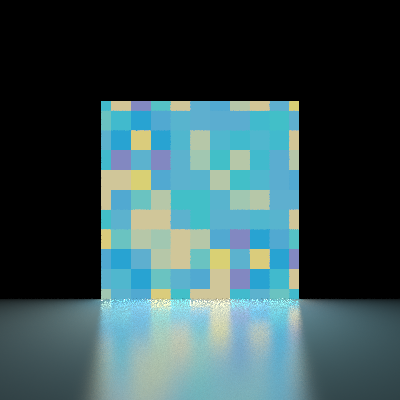
\includegraphics[width=0.4\linewidth]{./img/output2500v2}
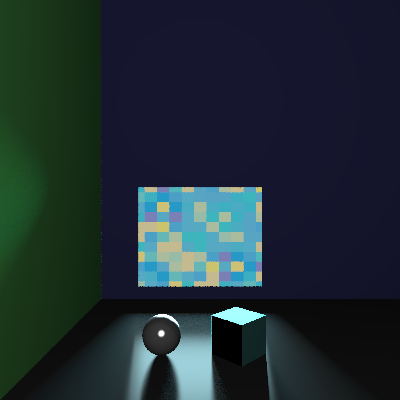
\includegraphics[width=0.4\linewidth]{./img/exp4}
\caption{Rendering of the pixelated window scene using 2500 samples per intersection point.}
\label{fig:output2500}
\end{figure}
Figure~\ref{fig:output2500} shows two images which where rendered using 2500 uniformly distributed samples on the light source. In the right image an additional point light has been added to illuminate the wall behind the area light source. Using this large amount of samples it can be assumed, that the solution of the rendering equation has converged to a point where the solution does not vary anymore. Using a similar low resolution images with 200 by 200 pixels, a series of experiments is conducted to verify the quality of the implemented methods. Using the importance function 
\begin{equation}
f_{\text{imp}} = G \cdot ( f_{\text{diffuse}} + f_{\text{specular}} ).
\label{eq:impfun1}
\end{equation}
The scene shown in figure~\ref{fig:output2500} has been computed hundred and fifty times with the number of area light samples linearly increasing.
\begin{figure}
\centering
% This file was created by matlab2tikz.
% Minimal pgfplots version: 1.3
%
%The latest updates can be retrieved from
%  http://www.mathworks.com/matlabcentral/fileexchange/22022-matlab2tikz
%where you can also make suggestions and rate matlab2tikz.
%
\documentclass[tikz]{standalone}
\usepackage{pgfplots}
\usepackage{grffile}
\pgfplotsset{compat=newest}
\usetikzlibrary{plotmarks}
\usepackage{amsmath}

\begin{document}
\definecolor{mycolor1}{rgb}{0.00000,0.44700,0.74100}%
\definecolor{mycolor2}{rgb}{0.85000,0.32500,0.09800}%
%
\begin{tikzpicture}

\begin{axis}[%
width=2.0in,
height=1.5in,
scale only axis,
xmin=0,
xmax=151,
ymin=0,
ymax=400,
xlabel={\#samples},
ylabel={mse}
]
\addplot [color=mycolor1,solid,forget plot]
  table[row sep=crcr]{%
1	358.66803333332\\
2	258.584783333324\\
3	216.888141666659\\
4	182.897900000007\\
5	166.240216666673\\
6	148.795108333339\\
7	134.154766666671\\
8	130.638983333338\\
9	117.809708333338\\
10	107.959383333338\\
11	106.908683333337\\
12	100.820016666663\\
13	92.6108083333298\\
14	89.2764666666632\\
15	88.0281499999964\\
16	84.1658083333301\\
17	80.3838166666632\\
18	77.7992499999969\\
19	77.1736916666636\\
20	73.5208166666636\\
21	72.4258249999972\\
22	68.700541666664\\
23	67.1192249999973\\
24	65.8873749999974\\
25	65.624908333331\\
26	65.4526249999974\\
27	62.6196749999978\\
28	59.8101833333312\\
29	60.7436916666642\\
30	58.129399999998\\
31	59.7129499999976\\
32	57.5551833333312\\
33	54.788199999998\\
34	54.798399999998\\
35	53.9502749999981\\
36	52.8570916666661\\
37	52.1957250000018\\
38	50.6694083333353\\
39	50.809083333335\\
40	49.5735083333347\\
41	49.6295083333351\\
42	49.1767583333351\\
43	46.7012916666684\\
44	45.725408333335\\
45	45.8570750000016\\
46	44.9244416666683\\
47	45.749258333335\\
48	45.5932166666687\\
49	44.6747416666682\\
50	44.4655500000017\\
51	41.6993250000014\\
52	42.6525833333351\\
53	44.3551333333347\\
54	41.1094916666683\\
55	40.5721916666681\\
56	40.7818500000014\\
57	40.4833333333348\\
58	41.2374333333349\\
59	40.6727250000014\\
60	38.2899666666681\\
61	39.6820416666681\\
62	38.3537000000014\\
63	37.9004083333348\\
64	38.8455000000015\\
65	39.9783500000014\\
66	37.9642500000015\\
67	35.9509583333346\\
68	35.4008500000013\\
69	37.1370250000013\\
70	34.9223166666679\\
71	36.9137333333347\\
72	35.6860250000014\\
73	37.4812916666681\\
74	37.1362583333345\\
75	34.9369833333345\\
76	33.1368666666677\\
77	36.653266666668\\
78	34.3618666666678\\
79	34.5482583333346\\
80	34.6478750000012\\
81	32.8031083333343\\
82	34.8950333333345\\
83	33.8877583333344\\
84	32.0820000000009\\
85	33.7148333333345\\
86	31.6101083333344\\
87	32.0522000000011\\
88	31.9836416666676\\
89	31.996175000001\\
90	32.682650000001\\
91	33.6024083333344\\
92	31.5365083333343\\
93	32.2464666666679\\
94	30.6462666666677\\
95	32.7104166666678\\
96	31.4869583333342\\
97	31.3221166666677\\
98	32.2380416666676\\
99	29.8472666666675\\
100	31.0600750000011\\
101	28.9802166666676\\
102	32.0539083333341\\
103	30.4257666666675\\
104	29.7841083333342\\
105	29.6575583333339\\
106	30.2834250000008\\
107	28.6633416666674\\
108	31.1428333333343\\
109	27.1567083333341\\
110	29.3878166666674\\
111	29.6792833333341\\
112	28.9703416666675\\
113	28.1620750000007\\
114	28.1602333333342\\
115	27.576183333334\\
116	28.6972166666674\\
117	29.0041083333341\\
118	27.1292750000008\\
119	28.2602666666675\\
120	29.1854166666675\\
121	27.8439500000008\\
122	26.247916666666\\
123	27.7680750000006\\
124	28.3610916666676\\
125	27.003783333334\\
126	26.7151000000005\\
127	26.6806750000004\\
128	27.708658333334\\
129	26.251816666666\\
130	25.4898916666659\\
131	26.2869083333328\\
132	28.186383333334\\
133	26.8427166666674\\
134	26.3219833333328\\
135	26.8339416666673\\
136	26.1574749999991\\
137	27.3697166666671\\
138	27.3866333333339\\
139	24.7993916666659\\
140	25.0228249999993\\
141	26.0116999999994\\
142	25.3358499999993\\
143	24.8282749999994\\
144	26.0334416666661\\
145	25.8605333333326\\
146	24.3936833333326\\
147	25.5006583333326\\
148	25.440266666666\\
149	26.7453916666672\\
150	26.3545916666663\\
151	25.1443333333328\\
};
\addplot [color=mycolor2,solid,forget plot]
  table[row sep=crcr]{%
1	132.807300000005\\
2	80.5151083333303\\
3	60.2227166666641\\
4	52.268083333335\\
5	47.3073500000016\\
6	41.8366916666681\\
7	40.0855583333348\\
8	35.6301666666679\\
9	34.1692083333345\\
10	34.1810583333346\\
11	31.4352166666678\\
12	31.4375333333343\\
13	30.1467750000008\\
14	27.7637750000008\\
15	28.0265916666673\\
16	25.0676249999993\\
17	27.0977583333339\\
18	24.865766666666\\
19	23.8419166666661\\
20	24.3815249999994\\
21	23.7033833333327\\
22	22.7558083333327\\
23	23.3504333333328\\
24	22.5110833333328\\
25	21.6344416666662\\
26	20.9164333333328\\
27	22.7039916666661\\
28	21.526108333333\\
29	20.8254666666662\\
30	20.5811916666662\\
31	20.2313333333329\\
32	19.6059999999996\\
33	21.1148833333329\\
34	19.1610749999997\\
35	20.0324166666664\\
36	20.1737999999996\\
37	19.8875916666664\\
38	19.2146666666664\\
39	17.3990666666664\\
40	18.4694249999998\\
41	18.4880166666665\\
42	17.9866833333331\\
43	19.2773749999997\\
44	17.5538583333332\\
45	17.7401583333331\\
46	18.5079583333332\\
47	17.4404666666666\\
48	16.9430083333333\\
49	16.9227666666666\\
50	15.784525\\
51	17.6963749999998\\
52	16.293\\
53	16.8767416666666\\
54	17.1609249999999\\
55	15.768825\\
56	15.7751166666666\\
57	16.0165916666667\\
58	16.7480916666667\\
59	15.9929166666666\\
60	14.5501166666667\\
61	15.6488166666666\\
62	16.2097166666667\\
63	15.1597083333334\\
64	15.8604916666666\\
65	15.526825\\
66	14.5090166666668\\
67	15.1548833333333\\
68	15.3188250000001\\
69	14.5389250000001\\
70	14.6468666666668\\
71	14.3129666666668\\
72	14.9357166666667\\
73	14.4025000000001\\
74	14.6659833333335\\
75	15.2488833333334\\
76	14.5714583333335\\
77	14.8407166666668\\
78	14.5292750000002\\
79	13.6726416666669\\
80	14.8901833333335\\
81	14.7780000000002\\
82	14.8228166666667\\
83	13.9361833333335\\
84	14.1400166666669\\
85	15.1674500000003\\
86	13.6336833333336\\
87	13.9685000000003\\
88	14.2259833333335\\
89	14.5413583333335\\
90	13.6190083333335\\
91	13.9811916666669\\
92	13.0629333333333\\
93	12.9143583333334\\
94	12.0586166666667\\
95	13.3817250000003\\
96	13.1898000000004\\
97	13.0094583333334\\
98	13.8996750000003\\
99	14.0729500000002\\
100	13.7628250000003\\
101	13.9294750000004\\
102	12.3505750000001\\
103	12.87995\\
104	12.8130250000001\\
105	14.0944750000002\\
106	12.1505416666667\\
107	14.302916666667\\
108	12.4474916666666\\
109	12.0663166666667\\
110	13.6847583333337\\
111	11.6810333333333\\
112	12.14985\\
113	13.0972583333334\\
114	13.02215\\
115	12.5515416666667\\
116	12.203475\\
117	13.1813083333338\\
118	12.5184916666667\\
119	12.2224083333333\\
120	11.6571916666667\\
121	11.9453416666667\\
122	12.9267583333333\\
123	12.9689416666667\\
124	12.896575\\
125	13.3395250000004\\
126	12.9715333333333\\
127	12.5391666666666\\
128	13.2489166666671\\
129	12.3019666666667\\
130	11.8484666666667\\
131	11.9439416666667\\
132	11.8308583333334\\
133	12.8942916666666\\
134	11.197825\\
135	11.5128083333333\\
136	13.4315000000003\\
137	11.452325\\
138	12.10755\\
139	12.2943833333333\\
140	11.6187249999999\\
141	10.5413916666666\\
142	12.5339416666667\\
143	12.295275\\
144	12.4880583333333\\
145	11.8696083333334\\
146	12.169375\\
147	11.9169083333333\\
148	12.614725\\
149	12.2440583333333\\
150	12.0916416666666\\
151	11.8550166666666\\
};
\end{axis}
\end{tikzpicture}%
\end{document}
% This file was created by matlab2tikz.
% Minimal pgfplots version: 1.3
%
%The latest updates can be retrieved from
%  http://www.mathworks.com/matlabcentral/fileexchange/22022-matlab2tikz
%where you can also make suggestions and rate matlab2tikz.
%
\documentclass[tikz]{standalone}
\usepackage{pgfplots}
\usepackage{grffile}
\pgfplotsset{compat=newest}
\usetikzlibrary{plotmarks}
\usepackage{amsmath}

\begin{document}
\definecolor{mycolor1}{rgb}{0.00000,0.44700,0.74100}%
\definecolor{mycolor2}{rgb}{0.85000,0.32500,0.09800}%
%
\begin{tikzpicture}

\begin{axis}[%
width=2.0in,
height=2.0in,
scale only axis,
xmin=0,
xmax=160,
ymin=0,
xlabel={\#samples},
ylabel={time [s]},
ymax=12
]
\addplot [color=mycolor1,solid,forget plot]
  table[row sep=crcr]{%
1	0.73\\
2	0.73\\
3	0.84\\
4	1.3\\
5	1.34\\
6	1.36\\
7	1.54\\
8	1.53\\
9	1.44\\
10	1.62\\
11	1.54\\
12	1.61\\
13	1.7\\
14	1.87\\
15	1.9\\
16	2.01\\
17	2.21\\
18	1.97\\
19	2.11\\
20	1.97\\
21	2.36\\
22	2.35\\
23	2.43\\
24	2.41\\
25	2.44\\
26	3.1\\
27	2.51\\
28	2.59\\
29	2.83\\
30	2.92\\
31	2.76\\
32	2.63\\
33	2.96\\
34	2.67\\
35	2.88\\
36	2.76\\
37	2.74\\
38	3.78\\
39	3.67\\
40	3.45\\
41	3.87\\
42	3.2\\
43	3.42\\
44	3.47\\
45	3.95\\
46	3.56\\
47	3.89\\
48	3.49\\
49	4.56\\
50	3.9\\
51	4.45\\
52	4.33\\
53	5.06\\
54	4.48\\
55	4.34\\
56	4.83\\
57	4.45\\
58	4.26\\
59	4.5\\
60	4.6\\
61	5.5\\
62	5.25\\
63	4.81\\
64	5.08\\
65	4.43\\
66	5.2\\
67	4.89\\
68	4.68\\
69	5.09\\
70	5.32\\
71	5.07\\
72	4.72\\
73	5.71\\
74	4.96\\
75	5.39\\
76	5.05\\
77	5.34\\
78	5.69\\
79	5.99\\
80	5.94\\
81	5.96\\
82	6.89\\
83	6.13\\
84	5.3\\
85	5.62\\
86	6.21\\
87	6.09\\
88	6.38\\
89	5.93\\
90	6.54\\
91	7.45\\
92	6.3\\
93	7.17\\
94	6.95\\
95	7.51\\
96	5.78\\
97	7.47\\
98	6.15\\
99	6.91\\
100	6.39\\
101	7.35\\
102	6.89\\
103	8.6\\
104	8.12\\
105	7.3\\
106	7.31\\
107	6.95\\
108	7.14\\
109	7.03\\
110	7.05\\
111	7.02\\
112	7.41\\
113	8.34\\
114	6.94\\
115	8.53\\
116	7.61\\
117	8.06\\
118	7.63\\
119	8.28\\
120	8.38\\
121	8.63\\
122	8.05\\
123	7.94\\
124	8.89\\
125	8.43\\
126	8.42\\
127	8.42\\
128	7.73\\
129	8.4\\
130	9.08\\
131	8.61\\
132	9.32\\
133	9.49\\
134	9.46\\
135	8.76\\
136	8.91\\
137	10.9\\
138	9.51\\
139	9.05\\
140	9.19\\
141	9.39\\
142	8.61\\
143	8.85\\
144	9.32\\
145	8.92\\
146	10.1\\
147	9.67\\
148	9.45\\
149	8.32\\
150	10.4\\
151	10\\
};
\addplot [color=mycolor2,solid,forget plot]
  table[row sep=crcr]{%
1	1.87\\
2	1.73\\
3	1.99\\
4	2.22\\
5	2.24\\
6	2.36\\
7	2.26\\
8	2.52\\
9	2.75\\
10	2.41\\
11	2.21\\
12	2.3\\
13	2.75\\
14	2.73\\
15	2.98\\
16	3.03\\
17	3.03\\
18	3.32\\
19	3.18\\
20	3.23\\
21	3.28\\
22	3.58\\
23	3.4\\
24	3.42\\
25	3.33\\
26	3.71\\
27	3.41\\
28	3.27\\
29	3.39\\
30	4.12\\
31	3.52\\
32	3.58\\
33	4.21\\
34	3.74\\
35	4.14\\
36	3.79\\
37	3.69\\
38	4.08\\
39	4.01\\
40	4.38\\
41	4.83\\
42	4.28\\
43	4.84\\
44	4.71\\
45	4.19\\
46	4.48\\
47	4.38\\
48	4.76\\
49	4.86\\
50	4.76\\
51	4.38\\
52	4.89\\
53	5.21\\
54	4.57\\
55	5.13\\
56	5.91\\
57	5.92\\
58	4.77\\
59	5.4\\
60	4.96\\
61	4.9\\
62	6.55\\
63	5.4\\
64	6.42\\
65	5.9\\
66	5.32\\
67	5.66\\
68	5.53\\
69	6.03\\
70	6.54\\
71	5.56\\
72	6.84\\
73	6.23\\
74	6.29\\
75	6.36\\
76	6.06\\
77	6.33\\
78	6.16\\
79	6.66\\
80	6.31\\
81	6.31\\
82	6.66\\
83	7.01\\
84	6.31\\
85	7.43\\
86	6.16\\
87	6.23\\
88	6.77\\
89	7.84\\
90	6.2\\
91	6.2\\
92	6.77\\
93	6.47\\
94	7.2\\
95	6.56\\
96	7.27\\
97	7.38\\
98	7.82\\
99	7.68\\
100	7.03\\
101	7.66\\
102	6.91\\
103	7.08\\
104	7.38\\
105	7.61\\
106	6.97\\
107	7.74\\
108	7.26\\
109	7.69\\
110	8.75\\
111	7.36\\
112	7.18\\
113	6.94\\
114	7.31\\
115	7.42\\
116	7.65\\
117	7.45\\
118	7.28\\
119	7.93\\
120	8.94\\
121	8.91\\
122	8.6\\
123	8.54\\
124	8.35\\
125	8.92\\
126	8.65\\
127	8.4\\
128	7.6\\
129	9.03\\
130	8.71\\
131	8.12\\
132	8.38\\
133	9.61\\
134	8.66\\
135	8.65\\
136	9.61\\
137	8.64\\
138	8.18\\
139	8.9\\
140	8.92\\
141	8.56\\
142	8.33\\
143	8.48\\
144	8.14\\
145	9.04\\
146	8.94\\
147	9.46\\
148	8.44\\
149	9.34\\
150	9.61\\
151	8.71\\
};
\end{axis}
\end{tikzpicture}%
\end{document}
\caption{Convergence and computation time of Monte-Carlo integration with (red) and without (blue) priority sampling for the scene shown in figure~\ref{fig:output2500} on the left. Using linearly increasing numbers of light source samples. }
\label{fig:impSampExp1}
\end{figure}
\begin{figure}
\centering
% This file was created by matlab2tikz.
% Minimal pgfplots version: 1.3
%
%The latest updates can be retrieved from
%  http://www.mathworks.com/matlabcentral/fileexchange/22022-matlab2tikz
%where you can also make suggestions and rate matlab2tikz.
%
\documentclass[tikz]{standalone}
\usepackage{pgfplots}
\usepackage{grffile}
\pgfplotsset{compat=newest}
\usetikzlibrary{plotmarks}
\usepackage{amsmath}

\begin{document}
\definecolor{mycolor1}{rgb}{0.00000,0.44700,0.74100}%
%
\begin{tikzpicture}

\begin{axis}[%
width=2.0in,
height=1.5in,
scale only axis,
xmin=0,
xmax=300,
ymin=10,
ymax=60,
xlabel={\#light-sources},
ylabel={mse}
]
\addplot [color=mycolor1,solid,mark=*,mark options={solid},forget plot]
  table[row sep=crcr]{%
1	43.2877583333349\\
4	55.0166749999981\\
9	46.2590500000016\\
16	38.6357583333343\\
25	33.1602750000006\\
36	27.7236500000002\\
49	23.4864416666662\\
64	22.0509416666664\\
81	20.692458333333\\
100	18.1443499999999\\
121	17.5964666666665\\
144	15.1360666666667\\
169	13.9261000000001\\
196	14.2328916666667\\
225	13.2898416666668\\
256	13.531675\\
};
\end{axis}
\end{tikzpicture}%
\end{document}
% This file was created by matlab2tikz.
% Minimal pgfplots version: 1.3
%
%The latest updates can be retrieved from
%  http://www.mathworks.com/matlabcentral/fileexchange/22022-matlab2tikz
%where you can also make suggestions and rate matlab2tikz.
%
\documentclass[tikz]{standalone}
\usepackage{pgfplots}
\usepackage{grffile}
\pgfplotsset{compat=newest}
\usetikzlibrary{plotmarks}
\usepackage{amsmath}

\begin{document}
\definecolor{mycolor1}{rgb}{0.00000,0.44700,0.74100}%
%
\begin{tikzpicture}

\begin{axis}[%
width=2.0in,
height=1.5in,
scale only axis,
xmin=0,
xmax=300,
ymin=3,
ymax=10,
xlabel={\#light-sources},
ylabel={time [s]}
]
\addplot [color=mycolor1,solid,mark=*,mark options={solid},forget plot]
  table[row sep=crcr]{%
1	3.47\\
4	3.11\\
9	3.46\\
16	3.12\\
25	3.37\\
36	3.57\\
49	3.94\\
64	4.07\\
81	5.25\\
100	5.1\\
121	7.71\\
144	7.89\\
169	8.4\\
196	9.18\\
225	9.07\\
256	9.98\\
};
\end{axis}
\end{tikzpicture}%
\end{document}
\caption{Convergence and computation time of Monte-Carlo integration priority sampling for the scene shown in figure~\ref{fig:output2500} on the left. For different numbers of light sources with 50 samples in total. }
\label{fig:impSampExp3}
\end{figure}
\begin{figure}
\centering
% This file was created by matlab2tikz.
% Minimal pgfplots version: 1.3
%
%The latest updates can be retrieved from
%  http://www.mathworks.com/matlabcentral/fileexchange/22022-matlab2tikz
%where you can also make suggestions and rate matlab2tikz.
%
\documentclass[tikz]{standalone}
\usepackage{pgfplots}
\usepackage{grffile}
\pgfplotsset{compat=newest}
\usetikzlibrary{plotmarks}
\usepackage{amsmath}

\begin{document}
\definecolor{mycolor1}{rgb}{0.00000,0.44700,0.74100}%
\definecolor{mycolor2}{rgb}{0.85000,0.32500,0.09800}%
%
\begin{tikzpicture}

\begin{axis}[%
width=2.5in,
height=1.5in,
scale only axis,
xlabel={\#samples},
ylabel={mse},
xmin=0,
xmax=120,
ymin=0,
ymax=150
]
\addplot [color=mycolor1,solid,forget plot]
  table[row sep=crcr]{%
1	147.232191666669\\
2	90.0739083333319\\
3	69.4578249999991\\
4	47.391033333334\\
5	43.9660083333339\\
6	35.9427750000005\\
7	34.0033250000003\\
8	32.0416666666669\\
9	25.4782749999997\\
10	26.5303833333338\\
11	23.4494916666663\\
12	21.2073166666664\\
13	20.3696916666664\\
14	19.9386666666664\\
15	18.4762916666666\\
16	16.4628666666666\\
17	17.5822916666666\\
18	15.3679083333333\\
19	16.3216416666665\\
20	18.7430249999999\\
21	16.7241249999998\\
22	14.3734749999998\\
23	14.8478999999999\\
24	13.8298999999998\\
25	15.1464333333331\\
26	13.4996916666664\\
27	12.6241000000002\\
28	14.1551499999998\\
29	14.0138749999999\\
30	13.8443083333332\\
31	13.4522416666665\\
32	12.9430333333335\\
33	13.6328583333331\\
34	12.8345583333334\\
35	12.4423750000001\\
36	9.87253333333342\\
37	11.0990250000002\\
38	11.6355000000001\\
39	9.50393333333339\\
40	10.4797000000001\\
41	11.9137250000001\\
42	11.77925\\
43	10.3094333333334\\
44	9.67507500000002\\
45	9.52396666666669\\
46	11.0755166666667\\
47	10.3592416666667\\
48	10.5560416666668\\
49	10.6581666666667\\
50	10.2305416666667\\
51	11.2276916666667\\
52	9.94687500000005\\
53	9.83200000000001\\
54	9.04138333333332\\
55	8.61455833333335\\
56	9.83080000000002\\
57	10.0299583333334\\
58	8.45465833333333\\
59	11.4692583333333\\
60	9.9287\\
61	9.88698333333336\\
62	9.4596333333333\\
63	9.09568333333336\\
64	9.25849166666666\\
65	11.943625\\
66	9.86868333333334\\
67	9.18576666666668\\
68	9.21629166666665\\
69	8.46070833333335\\
70	10.7330333333333\\
71	9.37040833333332\\
72	8.930125\\
73	8.15202500000001\\
74	6.89430833333335\\
75	9.21846666666667\\
76	9.48349999999996\\
77	8.63444999999997\\
78	8.56353333333334\\
79	7.84981666666665\\
80	8.93684999999996\\
81	8.29936666666668\\
82	9.58009999999997\\
83	7.98309166666668\\
84	9.11888333333331\\
85	9.12656666666665\\
86	8.68312499999996\\
87	7.39632500000002\\
88	6.93320000000001\\
89	11.3227083333333\\
90	8.13366666666664\\
91	9.60891666666666\\
92	8.41384166666661\\
93	8.67564166666665\\
94	8.99259999999998\\
95	8.63897500000002\\
96	9.84244999999999\\
97	9.04409999999997\\
98	8.72336666666664\\
99	9.12695833333328\\
100	6.73885833333331\\
101	8.53014999999996\\
};
\addplot [color=mycolor2,solid,forget plot]
  table[row sep=crcr]{%
1	88.4339166666652\\
2	71.3162249999988\\
3	59.2411250000004\\
4	54.8589083333376\\
5	52.313050000001\\
6	47.1871500000009\\
7	46.055175000001\\
8	45.2122250000009\\
9	42.959933333334\\
10	42.4038416666673\\
11	40.2524916666673\\
12	40.6008583333339\\
13	36.4580750000006\\
14	38.6087416666672\\
15	37.3395916666672\\
16	35.3495083333339\\
17	36.1741500000005\\
18	34.7821583333339\\
19	34.5885833333338\\
20	33.5354583333337\\
21	32.5697500000003\\
22	33.6338250000005\\
23	32.2519333333336\\
24	33.0984833333338\\
25	33.2858833333337\\
26	31.358375\\
27	31.8640083333335\\
28	29.9812416666663\\
29	30.7304333333333\\
30	31.6565083333334\\
31	29.7899249999996\\
32	32.3051916666669\\
33	30.4321916666666\\
34	29.4355833333323\\
35	27.759908333332\\
36	27.0950666666651\\
37	28.9347666666646\\
38	27.0622499999982\\
39	29.5476583333326\\
40	28.5656583333312\\
41	29.2037749999982\\
42	26.5827083333321\\
43	26.3082833333328\\
44	25.578333333333\\
45	26.2622499999996\\
46	27.9313833333319\\
47	27.2526749999988\\
48	26.9620833333315\\
49	25.8728999999997\\
50	24.7568083333331\\
51	25.0479083333331\\
52	26.5112749999989\\
53	25.8651833333331\\
54	24.291183333333\\
55	26.3689749999994\\
56	25.4658249999997\\
57	25.1871999999998\\
58	25.4525916666664\\
59	24.1431249999998\\
60	24.8142833333331\\
61	26.7697416666649\\
62	26.2295916666664\\
63	23.4912416666665\\
64	24.9160749999998\\
65	24.9948249999998\\
66	22.7636416666665\\
67	22.6848916666665\\
68	25.9860166666664\\
69	23.2209249999998\\
70	22.1747666666664\\
71	23.4937249999998\\
72	24.4664999999998\\
73	22.6529666666665\\
74	24.1107583333331\\
75	22.9035666666665\\
76	23.9216333333331\\
77	22.3706833333332\\
78	23.9021666666665\\
79	23.9134916666665\\
80	23.7637916666665\\
81	23.1775249999998\\
82	22.9618333333332\\
83	23.6968166666665\\
84	24.3271666666665\\
85	22.8132999999999\\
86	22.8026749999999\\
87	23.3020583333332\\
88	23.0031333333332\\
89	21.5461249999998\\
90	23.9589666666666\\
91	21.3867499999999\\
92	20.9766583333333\\
93	23.4005083333332\\
94	19.9074166666666\\
95	23.5974333333332\\
96	22.1976833333333\\
97	23.1644166666666\\
98	22.6627749999999\\
99	20.6210833333333\\
100	20.3840499999999\\
101	22.9414583333332\\
};
\end{axis}
\end{tikzpicture}%
\end{document}
% This file was created by matlab2tikz.
% Minimal pgfplots version: 1.3
%
%The latest updates can be retrieved from
%  http://www.mathworks.com/matlabcentral/fileexchange/22022-matlab2tikz
%where you can also make suggestions and rate matlab2tikz.
%
\documentclass[tikz]{standalone}
\usepackage{pgfplots}
\usepackage{grffile}
\pgfplotsset{compat=newest}
\usetikzlibrary{plotmarks}
\usepackage{amsmath}

\begin{document}
\definecolor{mycolor1}{rgb}{0.00000,0.44700,0.74100}%
\definecolor{mycolor2}{rgb}{0.85000,0.32500,0.09800}%
%
\begin{tikzpicture}

\begin{axis}[%
width=2.0in,
height=1.5in,
scale only axis,
xmin=0,
xmax=100,
ymin=0,
ymax=14,
xlabel={\#samples},
ylabel={time [s]}
]
\addplot [color=mycolor1,solid,forget plot]
  table[row sep=crcr]{%
1	0.88\\
2	0.97\\
3	1.09\\
4	1.3\\
5	1.57\\
6	1.74\\
7	1.69\\
8	1.77\\
9	2.14\\
10	1.97\\
11	2.03\\
12	2.05\\
13	2.41\\
14	2.17\\
15	2.48\\
16	2.39\\
17	2.49\\
18	2.86\\
19	2.74\\
20	2.76\\
21	2.74\\
22	3.21\\
23	3.03\\
24	3.15\\
25	3.1\\
26	3.04\\
27	3.11\\
28	3.1\\
29	3.3\\
30	3.19\\
31	3.45\\
32	3.54\\
33	3.56\\
34	3.63\\
35	3.56\\
36	3.73\\
37	3.98\\
38	3.94\\
39	4.02\\
40	4\\
41	4.33\\
42	4.21\\
43	4.27\\
44	4.37\\
45	4.64\\
46	4.73\\
47	5.03\\
48	4.57\\
49	4.79\\
50	4.87\\
51	4.86\\
52	5.59\\
53	5.14\\
54	5.09\\
55	5.23\\
56	5.66\\
57	5.27\\
58	5.46\\
59	5.68\\
60	5.56\\
61	5.78\\
62	5.73\\
63	6.1\\
64	5.79\\
65	5.96\\
66	6.17\\
67	6.4\\
68	6.19\\
69	6.28\\
70	6.5\\
71	7.14\\
72	7\\
73	7.2\\
74	6.62\\
75	7.93\\
76	7.41\\
77	7.22\\
78	7.93\\
79	8.41\\
80	7.79\\
81	7.37\\
82	7.52\\
83	7.21\\
84	7.5\\
85	7.47\\
86	7.53\\
87	7.92\\
88	7.65\\
89	8.17\\
90	7.87\\
91	7.99\\
92	8.7\\
93	8.14\\
94	8.11\\
95	8.3\\
96	8.31\\
97	8.51\\
98	9.3\\
99	9.64\\
};
\addplot [color=mycolor2,solid,forget plot]
  table[row sep=crcr]{%
1	3.6\\
2	3.72\\
3	4.57\\
4	4.47\\
5	4.24\\
6	4.06\\
7	4.26\\
8	4.58\\
9	4.45\\
10	5.05\\
11	4.69\\
12	4.43\\
13	4.79\\
14	5.36\\
15	4.93\\
16	4.84\\
17	4.65\\
18	5.18\\
19	5\\
20	5.36\\
21	5.18\\
22	5.3\\
23	5.43\\
24	6.03\\
25	6.47\\
26	5.48\\
27	5.97\\
28	6.49\\
29	6.04\\
30	6.16\\
31	5.97\\
32	6.84\\
33	6.5\\
34	6.37\\
35	6.86\\
36	6.3\\
37	6.15\\
38	6.91\\
39	6.21\\
40	7.08\\
41	7.29\\
42	6.91\\
43	6.46\\
44	6.4\\
45	6.63\\
46	6.88\\
47	7.26\\
48	8.32\\
49	7.09\\
50	7.15\\
51	7.34\\
52	7.33\\
53	7.7\\
54	7.45\\
55	7.34\\
56	7.54\\
57	7.51\\
58	7.46\\
59	7.47\\
60	8.78\\
61	7.61\\
62	7.8\\
63	8.18\\
64	7.97\\
65	7.66\\
66	7.76\\
67	7.9\\
68	8.66\\
69	7.98\\
70	8.14\\
71	8.09\\
72	8.47\\
73	8.62\\
74	8.8\\
75	8.54\\
76	8.93\\
77	9.32\\
78	8.43\\
79	8.98\\
80	8.9\\
81	9.22\\
82	8.75\\
83	9.01\\
84	9.53\\
85	11.47\\
86	9.51\\
87	9.77\\
88	9.29\\
89	9.16\\
90	9.65\\
91	9.63\\
92	9.89\\
93	9.72\\
94	10.77\\
95	10.43\\
96	9.62\\
97	9.55\\
98	13.1\\
99	10.25\\
};
\end{axis}
\end{tikzpicture}%
\end{document}
\caption{Convergence of Monte-Carlo integration with (red) and without (blue) priority sampling for the scene shown in figure~\ref{fig:output2500} on the right. Using linearly increasing numbers of light source samples. }
\label{fig:impSampExp2}
\end{figure}
The results are shown in figure~\ref{fig:impSampExp1}. With no shadows in the image the importance sampling algorithm does deliver better results in comparison to pure Monte-Carlo estimation for any number of samples tried.
Increasing the number of partial light sources leads to faster convergence, at the expense of longer computation times as illustrated in the plots in~\ref{fig:impSampExp3}. 
In figure~\ref{fig:impSampExp2} results of the scene shown in figure~\ref{fig:output2500} on the right are shown. With a significant part of the plain covered by shadows importance sampling looses it's edge. It produced results on par with uniformly distributed samples, while taking more time on average. This is probably due to the fact that this importance function used so far does only take geometry into account, and assumes $V(\mathbf{p},\mathbf{p}') = 1$, so it does not allocate fewer samples in areas which lie in the shadow of the two new objects and do not contribute to the solution. 
In general the importance sampling method implemented here could be improved further, for example by finding better importance functions, which in turn could yield better sample distributions leading to faster convergence. It has been shown that the importance sampling method implemented here
works better than plain Monte-Carlo integration for scenes where not too much area is covered by shadows and small sample numbers. For larger numbers of samples the two methods deliver similar results, depending on the arrangement of objects plain Monte-Carlo can be the better choice due to its faster execution time.  
\begin{figure}
\centering
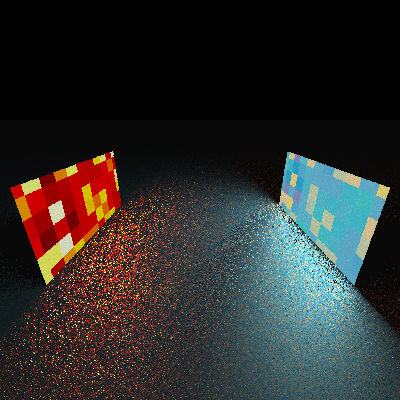
\includegraphics[width=0.3\linewidth]{./img/twoAI/1}
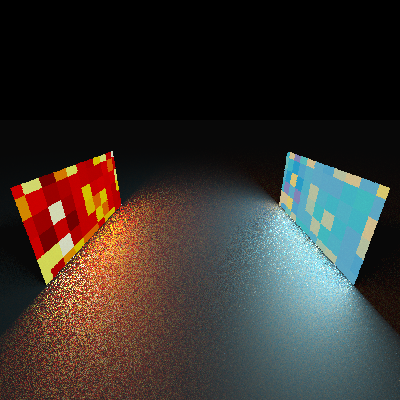
\includegraphics[width=0.3\linewidth]{./img/twoAI/11}
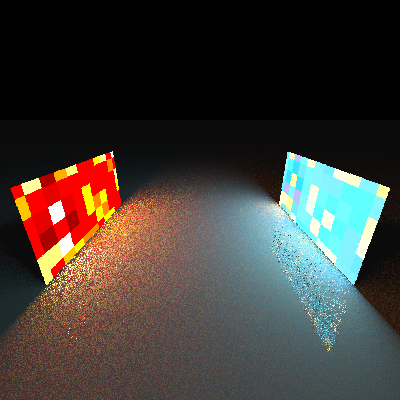
\includegraphics[width=0.3\linewidth]{./img/twoAI/21}
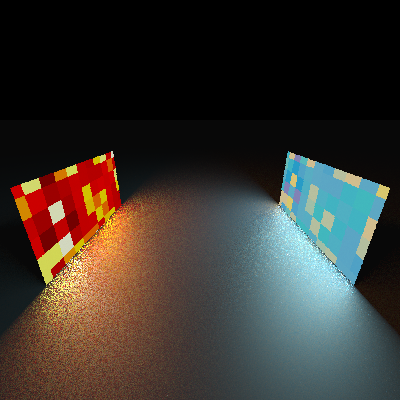
\includegraphics[width=0.3\linewidth]{./img/twoAI/51}
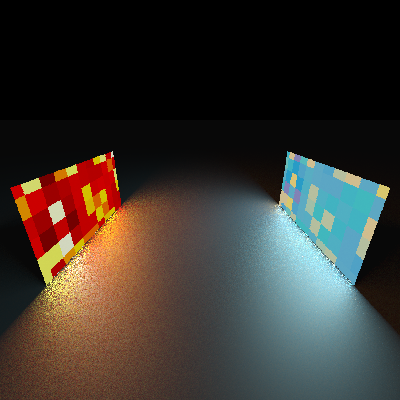
\includegraphics[width=0.3\linewidth]{./img/twoAI/101}
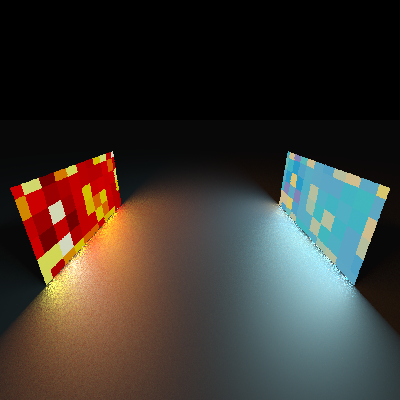
\includegraphics[width=0.3\linewidth]{./img/twoAI/501}
\caption{Plain Monte Carlo (red) and importance sampled Monte-Carlo with 121 subdivisions (blue). Results for 1,11,21,51,101 and 501 samples are shown from left to right. The plane material is given by $\rho_{\text{diff}} = 0.8,  \rho_{\text{spec}} = 0.2, f_{\text{ct}}(0.015,0.01)$.}
\label{fig:twoLight}
\end{figure}

Figure~\ref{fig:twoLight} shows a uniformly sampled Monte-Carlo light source in red on the left and a importance sampled Monte-Carlo light source on the right. The top row shows how well the importance sampling does in terms of variance reduction for small light source sample numbers. Even for only one area light sample per intersection points the contours of the specular reflection are visible. For higher numbers of area light sampled the difference becomes less significant.

\section{Conclusion}
In this project a ray tracer consisting of more then six-thousand lines of code has been written. Another thousand lines have been written from scratch in python, but that version had to be abandoned out of speed concerns. The Java version of the ray tracer covers key areas of the course, generally the implemented features work, but much room for further improvement still remains. The tree generation process especially for SAH-Trees could be optimized further, currently SAH beats all the other methods in terms of rendering time, but takes longer overall for complex wavefront objects consisting of large numbers of triangles, because the tree generation is slow.  Importance sampling works as well but currently takes only the scene geometry into account. An improved version could use the texture information to converge even faster. 



